\thispagestyle{plain}
\section{Composición y estructura de distintos tipos de sustancias}

\boxabstract{Aprendizajes esperados:}{
    \begin{itemize}
        \item Representa y diferencia mediante esquemas, modelos y
              simbología química, elementos y compuestos, así como
              átomos y moléculas.
        \item Explica y predice propiedades físicas de los materiales
              con base en modelos submicroscópicos sobre la
              estructura de átomos, moléculas o iones, y sus
              interacciones electrostáticas.
    \end{itemize}
}
%\newpage

\subsection{Qué tipos de partículas se forman al combinar los átomos?}
\begin{boxK}
    \begin{enumerate}
        \item La tabla \ref{tab:tabla_sustancias} presenta ejemplos de sustancias comunes. En la unidad 1 realizaste experimentos con algunas de ellas y estudiaste sus propiedades.
              \begin{figure}[H]
                  \centering
                  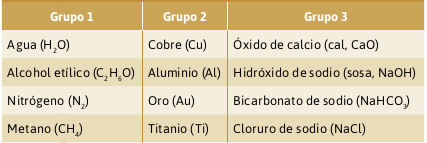
\includegraphics[width=.6\textwidth]{tabla_sustancias.png}
                  \captionof{table}{Grupos de sustancias}
                  \label{tab:tabla_sustancias}
              \end{figure}
        \item Describe propiedades comunes a las sustancias de cada grupo. Considera su apariencia física, estado de agregación, solubilidad en agua y conductividad eléctrica.
        \item Considera la composición y estructura de las partículas que componen las sustancias de cada grupo, y plantea hipótesis sobre qué genera esas propiedades.
        \item Comparte tus ideas con tus compañeros de grupo y reflexiona ¿coinciden las propiedades que observaste con las que ellos identificaron? Complementen sus descripciones.
    \end{enumerate}
\end{boxK}

\subsubsection{Los tipos de sustancias y sus diferencias}
Cada sustancia tiene propiedades diferentes, por ejemplo, algunas son solubles
en agua y otras no, o algunas conducen la electricidad mientras otras son aislantes
eléctricos. Existen diversas maneras de clasificar las sustancias con base en sus
propiedades, y una de ellas se muestra en la tabla \ref{tab:tabla_sustancias2}.

\begin{figure}[H]
    \centering
    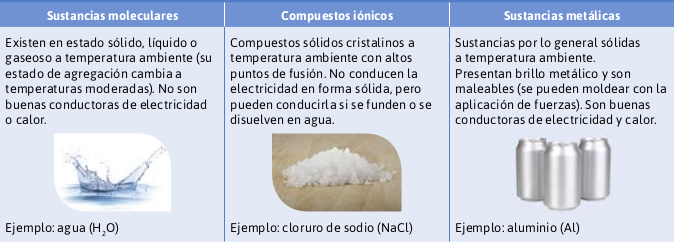
\includegraphics[width=\textwidth]{tabla_sustancias2.png}
    \captionof{table}{Tipos de sustancias y sus propiedades}
    \label{tab:tabla_sustancias2}
\end{figure}

\begin{boxK}
    Analiza y predice
    \begin{enumerate}
        \item Predice, con base en tus observaciones, experiencias y conocimientos adquiridos en este curso, a qué grupo
              (sustancias moleculares, compuestos iónicos o sustancias metálicas) pertenece cada uno de los siguientes materiales.
              Justifica tus predicciones de acuerdo con sus propiedades físicas.
              \begin{enumerate}
                  \item Plata (Ag)
                  \item Azúcar (C$_{12}$H$_{22}$O$_{11}$)
                  \item Carbonato de calcio (CaCO$_3$)
                  \item Acetona (C$_3$H$_6$O)
                  \item Nitrato de sodio (salitre, NaNO$_3$)
                  \item Hierro (Fe)
              \end{enumerate}
        \item Argumenta tus predicciones con tus compañeros.
    \end{enumerate}
\end{boxK}

Para explicar las propiedades de las sustancias moleculares, iónicas y metálicas, los científicos han propuesto
que las partículas que las constituyen tienen composición y estructura características. La estructura se refiere
a la manera en que los átomos o iones se agrupan. A continuación se describirán y analizarán las diferencias a
nivel nanoscópico entre estos tres grandes grupos de sustancias.



\subsubsection{Sustancias moleculares}

\begin{figure}[H]
    \centering
    \captionof{figure}{ Atracción y repulsión entre protones y electrones durante la formación de una molécula.}
    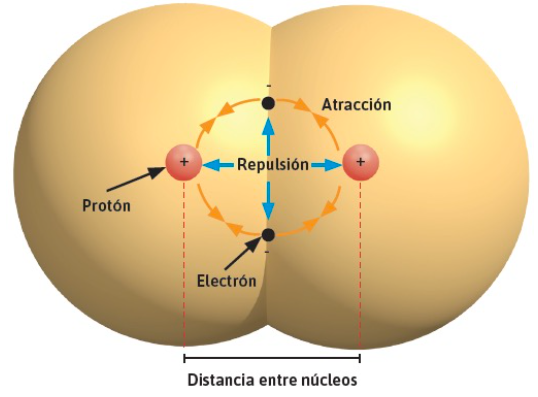
\includegraphics[width=.5\textwidth]{atraccion_repulsion.png}
    \label{fig:atraccion_repulsion}
\end{figure}

Para explicar que este tipo de sustancias no conduce la electricidad y tiene puntos de
ebullición y fusión relativamente bajos, se propuso que están constituidas por moléculas
neutras (su carga eléctrica neta es cero) que se forman cuando átomos del mismo o diferente
tipo se unen entre sí. Cada molécula se forma cuando dos o más átomos se acercan, y los
protones de uno atraen a los electrones de valencia del otro (figura \ref{tab:tabla_sustancias}). Esta fuerza
de atracción mantiene a los átomos juntos en la molécula.

Las \textbf{sustancias moleculares} son resultado de la combinación de elementos químicos conocidos
como \textbf{no metales}. Entre ellos se encuentran el hidrógeno y los elementos localizados en la
esquina superior derecha de la tabla periódica (figura \ref{tab:tabla_sustancias2}).
La unión entre dos átomos que forman una molécula por lo general se representa mediante
una línea, como se ilustra a continuación para la molécula de hidrógeno (H$_2$).

\begin{center}
    H - H
\end{center}

La línea entre los símbolos de los átomos representa la fuerza que los mantiene unidos.
A esta representación se le conoce como fórmula estructural, en este caso de la molécula
de hidrógeno, mientras que el símbolo H$_2$ se conoce como fórmula condensada.

\begin{figure}[H]
    \centering
    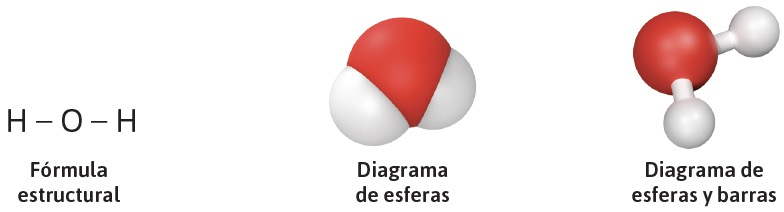
\includegraphics[width=0.8\textwidth]{esferas.jpg}
    \captionof{figure}{ Diferentes representaciones de la misma molécula. ¿Qué diferencias y semejanzas encuentras?}
    \label{fig:esferas}
\end{figure}

Algunos átomos de elementos no metálicos pueden unirse al mismo tiempo a más de un átomo.
Considera, por ejemplo, el caso de la molécula de agua: cada una tiene un átomo de oxígeno
unido a dos átomos de hidrógeno como se muestra en esta fórmula estructural:

\begin{center}
    H - O - H
\end{center}

Existen diversas formas de representar la unión de los átomos de las moléculas, y hoy en día,
con la ayuda de las computadoras, es posible generar imágenes tridimensionales de cualquier
molécula.

En la figura \ref{fig:esferas}, por ejemplo,
se ilustran algunas maneras de representar una molécula de agua (H$_2$O).

En los diagramas tridimensionales los átomos se representan como esferas. Los enlaces a
veces se muestran como barras que las conectan (diagramas de esferas y barras) o no se muestran de manera visible (diagramas de esferas).

Mediante el análisis de la composición química de múltiples sustancias moleculares,
se ha descubierto que cada tipo de átomo en general forma un número determinado de enlaces.
Por ejemplo, cada átomo de hidrógeno forma sólo un enlace con otros, mientras que cada
átomo de oxígeno forma dos enlaces.

El número de enlaces que cada tipo de átomo puede
formar se denomina capacidad de combinación del elemento o valencia. La figura \ref{fig:valencia}
muestra la valencia de los elementos no metálicos: la del hidrógeno es 1, lo cual
indica que este tipo de átomos sólo forma un enlace con otros; la del carbono es 4,
lo cual señala que este tipo de átomo típicamente forma cuatro enlaces con otros.

\begin{minipage}{.4\textwidth}
    \begin{figure}[H]
        \centering
        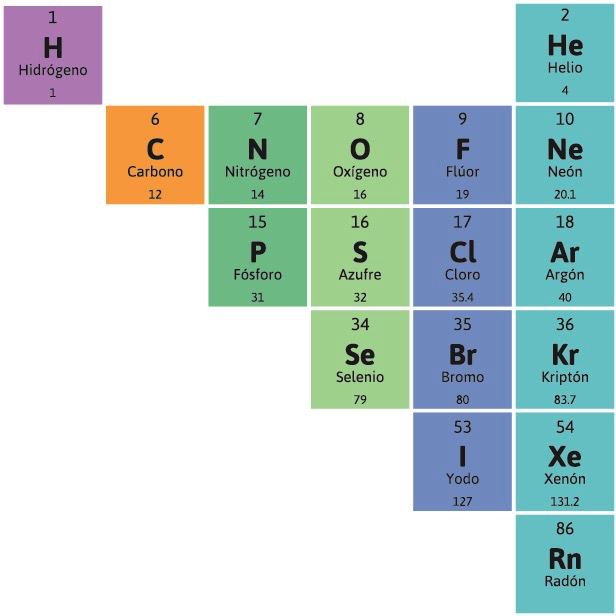
\includegraphics[width=0.5\textwidth]{no_metales.jpg}
        \label{fig:no_metales}
        \captionof{figure}{ Elementos no metálicos.}
    \end{figure}
\end{minipage}\hfill
\begin{minipage}{.4\textwidth}
    \begin{figure}[H]
        \centering
        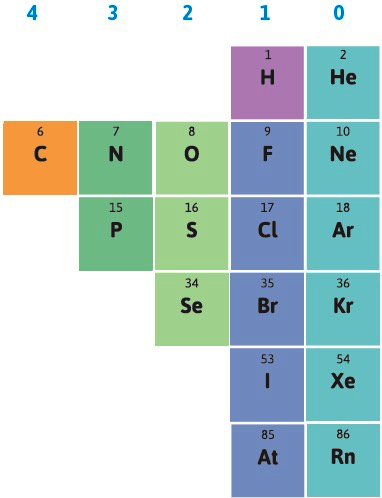
\includegraphics[width=0.5\textwidth]{valencia.jpg}
        \captionof{figure}{ Valencia (capacidad de combinación) de diferentes tipos de átomos no metálicos.}
        \label{fig:valencia}
    \end{figure}
\end{minipage}

La valencia de los elementos es una propiedad periódica; esto significa que los átomos de elementos de un mismo grupo o familia (columna) de la tabla periódica en general forman el mismo número de enlaces cuando se combinan con otros. Este comportamiento facilita la predicción de la composición química y estructura de las moléculas que resultan al combinar distintos tipos de átomos de elementos no metálicos.

\begin{boxK}
    Representa e infiere
    \begin{enumerate}
        \item Considera la valencia o capacidad de combinación de los diferentes átomos no metálicos y representa la fórmula estructural de las moléculas que se forman cuando:
              \begin{enumerate}
                  \item un átomo de carbono se combina con átomos de hidrógeno;
                  \item un átomo de nitrógeno se combina con átomos de hidrógeno;
                  \item un átomo de cloro se combina con átomos de hidrógeno.
              \end{enumerate}
        \item Escribe la fórmula condensada de las moléculas que se crean en cada caso. En esta fórmula primero se escribe el átomo que forma más enlaces.
        \item Compara y contrasta tus representaciones con las de algunos compañeros. Corríjanlas en caso de ser necesario.
    \end{enumerate}
\end{boxK}

En algunos casos, un átomo llega a formar más de un enlace con otro debido a que varios electrones de valencia de cada átomo son atraídos por los protones del otro. Por ejemplo, un átomo de carbono y uno de oxígeno pueden unirse con dos enlaces (enlace doble). En la molécula de dióxido de carbono, esto sucede como se ilustra a continuación.

\subsubsection{Ejercicios}
\begin{boxK}
    Relaciona la especie química con la cantidad de \textbf{protones} y \textbf{electrones de valencia}.\\

    \begin{minipage}{0.6\textwidth}
        \begin{enumerate}
            \item Las sustancias se representan con símbolos atómicos y líneas que simbolizan a los enlaces químicos.
            \item Esquema tridimensional en el que no es posible identificar a los enlaces químicos.
            \item Las sustancias se representan sólo con símbolos atómicos.
            \item Esquema tridimensional en el que es posible identificar a los enlaces químicos.
        \end{enumerate}
    \end{minipage}\hfill
    \begin{minipage}{0.3\textwidth}
        \begin{itemize}
            \item[\rule{1cm}{0.2mm}] Diagrama de esferas\\
            \item[\rule{1cm}{0.2mm}] Fórmula estructural\\
            \item[\rule{1cm}{0.2mm}] Fórmula condensada\\
            \item[\rule{1cm}{0.2mm}] Diagrama de esferas y barras\\
        \end{itemize}
    \end{minipage}

\end{boxK}

\begin{figure}[H]
    \centering
    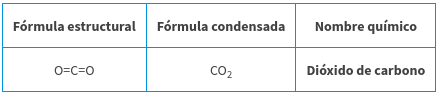
\includegraphics[width=0.6\textwidth]{formulas_co2.png}
    \label{fig:formulas_co2}
    % \captionof{figure}{  Valencia (capacidad de combinación) de diferentes tipos de átomos no metálicos.}
\end{figure}

Observa que en la fórmula estructural del dióxido de carbono el enlace doble se representa con dos líneas
paralelas entre los átomos. La fuerza de atracción entre los átomos unidos por un doble enlace es mayor
que la que existe entre aquellos unidos por un solo enlace.

\begin{figure}[H]
    \centering
    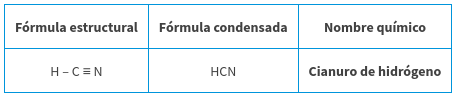
\includegraphics[width=0.6\textwidth]{formulas_hcn.png}
    \label{fig:formulas_hcn}
    % \captionof{figure}{  Valencia (capacidad de combinación) de diferentes tipos de átomos no metálicos.}
\end{figure}

Algunos átomos pueden formar entre ellos hasta tres enlaces (enlace triple),
como en la unión entre átomos de carbono y nitrógeno en el cianuro de hidrógeno,
un compuesto molecular muy tóxico. El enlace triple se representa con tres líneas
paralelas entre los átomos que se unen.

\begin{wrapfigure}{l}{0.45\textwidth}
    \centering
    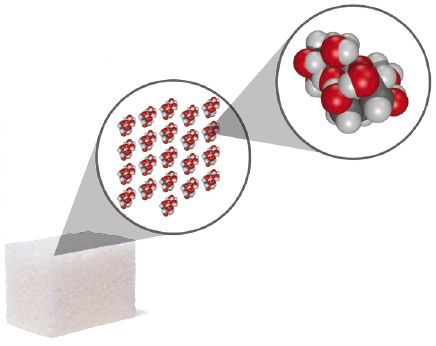
\includegraphics[width=0.7\linewidth]{azucar.jpg}
    \captionof{figure}{ Un cubo de azúcar esta constituido por miles de millones
        de moléculas de sacarosa, cada una de ellas con 45 átomos (C$_{12}$H$_{22}$O$_{11}$) .}
    \label{fig:azucar}
\end{wrapfigure}

Los átomos de elementos no metálicos se pueden unir para formar moléculas pequeñas,
como las de agua (H$_2$O) y dióxido de carbono (CO$_2$), pero también pueden formar moléculas con
decenas o centenas de átomos cada una. Considera, por ejemplo, los casos del octano (C$_8$H$_{18}$),
el componente principal de la gasolina, en el que cada molécula está compuesta por 26 átomos,
o el azúcar (también llamada sacarosa, C$_{12}$H$_{22}$O$_{11}$), con 45 átomos por molécula (figura \ref{fig:azucar}).

En nuestro mundo, una gran proporción de las sustancias naturales y sintéticas resulta de la
combinación de los siguientes elementos no metálicos: carbono (C), hidrógeno (H), oxígeno (O), nitrógeno
(N) y azufre (S). Veamos algunos ejemplos en la siguiente actividad.

\begin{minipage}{\textwidth}
    \begin{boxK}
        Investiga y comunica
        \begin{enumerate}
            \item Investiga la fórmula condensada y estructural de las moléculas que constituyen las siguientes sustancias.
                  \begin{enumerate}
                      \item Cafeína: sustancia estimulante en bebidas como el café y los refrescos.
                      \item Capsaicina: sustancia que causa la sensación picante de los chiles.
                      \item Alicina: sustancia responsable del olor del ajo.
                  \end{enumerate}
            \item Determina de qué tipos y de cuántos átomos en total se conforma cada molécula, y qué tipos de enlaces
                  (sencillos, dobles, o triples) establecen.
            \item Comparte los resultados de tu investigación con tus compañeros y verifíquenlos.
        \end{enumerate}
    \end{boxK}
\end{minipage}

\subsubsection{Sustancias metálicas}

\begin{figure}[H]
    \centering
    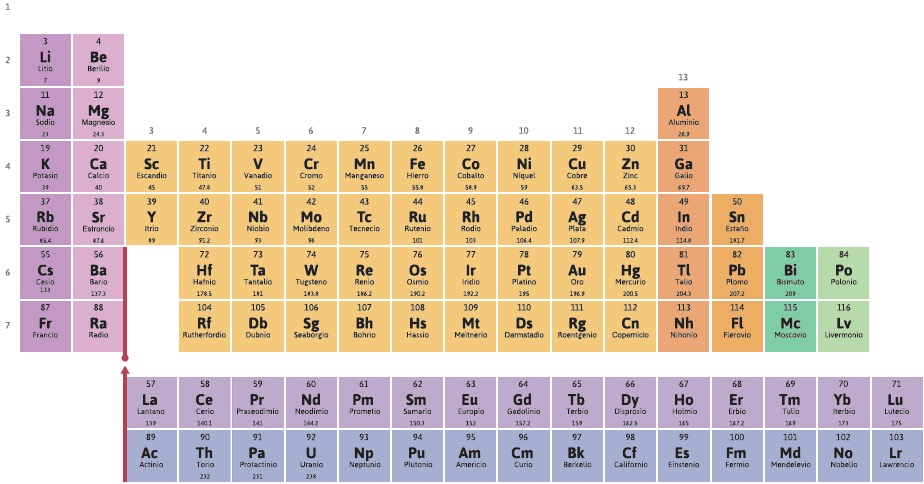
\includegraphics[width=.9\textwidth]{metales.jpg}
    \captionof{figure}{ Elementos metálicos.}
    \label{fig:metales}
\end{figure}

\begin{wrapfigure}{r}{0.5\textwidth}
    \centering
    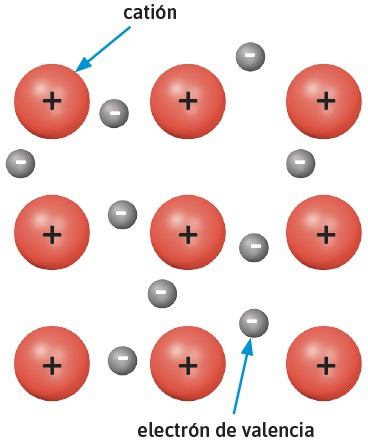
\includegraphics[width=0.4\linewidth]{electron_valencia.jpg}
    \captionof{figure}{ Representación del modelo de \emph{mar de electrones} para un metal.}
    \label{fig:electron_valencia}
\end{wrapfigure}

La mayoría de los elementos químicos en la tabla periódica son metálicos
(figura \ref{fig:metales}), cuyos átomos pierden sus electrones con relativa facilidad cuando interaccionan
entre sí o con otro tipo de átomos. Imagina que varios átomos de sodio (Na), un elemento metálico, interaccionan
unos con otros. Durante la interacción cada átomo pierde un electrón de valencia y forma un ion Na+; sin embargo,
los electrones de valencia no se transfieren de forma directa a otros átomos, sino que permanecen moviéndose alrededor
de todos los iones de sodio formados. Por ello se dice que se origina un \emph{mar de electrones}, en el
que los electrones de valencia se desplazan entre todos los iones del sistema (figura \ref{fig:electron_valencia}).
También hay que mencionar que los cationes y electrones permanecen unidos porque unos a otros se atraen debido a
su carga eléctrica, creando una \emph{red metálica}.


\begin{figure}[H]
    \centering
    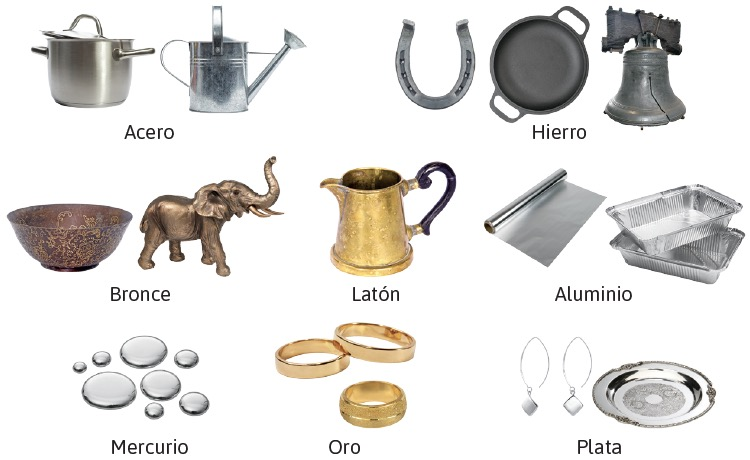
\includegraphics[width=0.6\textwidth]{metalicas.jpg}
    \captionof{figure}{ Diferentes tipos de sustancias metálicas.}
    \label{fig:metalicas}
\end{figure}

Como los electrones que forman el \emph{mar} se mueven con facilidad de un lado a otro, los metales
son buenos conductores de corriente eléctrica (esta corriente eléctrica es tan sólo el movimiento de
los electrones de valencia de un lugar a otro en el metal cuando en sus extremos se aplica una
diferencia de voltaje). El mar de electrones también permite que los metales sean buenos conductores
del calor, reflejen la luz y sean maleables (se puedan moldear sin romperse y hacer láminas).
La mayoría de los metales son sólidos a temperatura ambiente, aunque hay sustancias metálicas
líquidas, como el mercurio (Hg) (figura \ref{fig:metalicas}).

\begin{wrapfigure}{r}{0.4\textwidth}
    \centering
    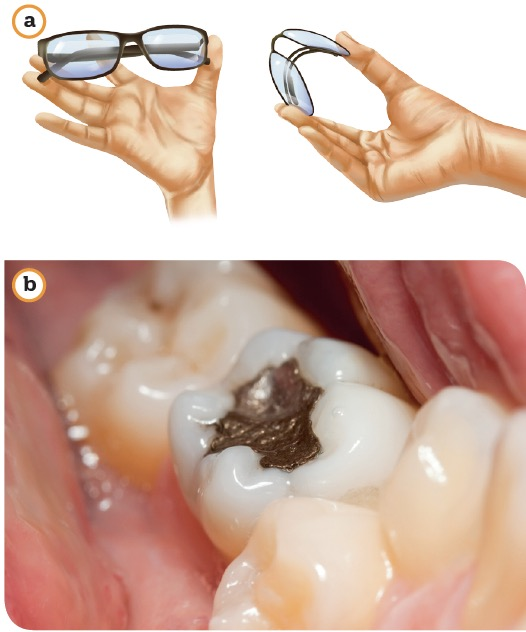
\includegraphics[width=0.4\textwidth]{metalicas2.jpg}
    \captionof{figure}{ Diferentes tipos de sustancias metálicas.}
    \label{fig:metalicas2}
\end{wrapfigure}

Los metales no forman compuestos químicos cuando se combinan con otros metales, tan sólo se mezclan.
Estas mezclas se llaman aleaciones, y los químicos e ingenieros en materiales han logrado
hacer mezclas metálicas con propiedades extraordinarias. La mayoría de los materiales metálicos
que cada día usamos está hecha de aleaciones, como el acero, el bronce, la alpaca, el peltre y
las amalgamas. Algunas de ellas tienen propiedades superplásticas, esto es, pueden estirarse
hasta alcanzar cien veces su longitud original sin romperse. Un ejemplo es la amalgama de zinalco,
una aleación de cinc (Zn) y aluminio (Al). Otras como el nitinol formado por la mezcla de níquel (Ni)
y titanio (Ti), originan materiales que recuperan su forma original después de deformarlos (figura \ref{fig:metalicas2}).

\begin{wrapfigure}{l}{0.3\textwidth}
    \centering
    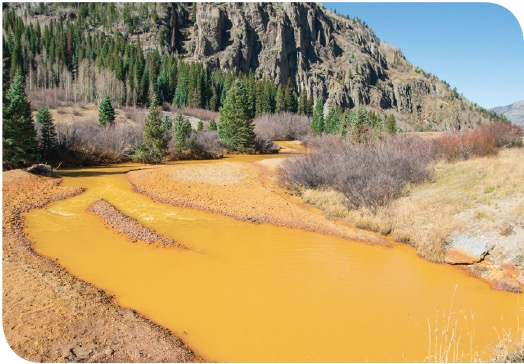
\includegraphics[width=0.3\textwidth]{metalicas3.jpg}
    \captionof{figure}{ Contaminación causada durante la extracción de hierro.
        El color rojizo se debe a especies oxidadas de hierro.}
    \label{fig:metalicas3}
\end{wrapfigure}

¿Imaginas tu vida sin materiales metálicos? Sin cobre (Cu) para fabricar los cables que conducen la
electricidad a la que conectas el televisor, sin la lata de aluminio (Al) maleable de tu bebida
favorita, sin el hierro (Fe) resistente pero con la elasticidad necesaria para construir casas y
edificios, sin el litio (Li) y el cadmio (Cd) de las pilas con las que funcionan los aparatos que
utilizas a diario, como en los teléfonos celulares. Sin duda es difícil concebir un mundo sin metales
porque no tendríamos materiales suficientes para sustituirlos.

En la actualidad, cada año se consumen miles de toneladas de diferentes tipos de metales,
dado que las aplicaciones tecnológicas los requieren; sin embargo, se trata de recursos
no renovables, y su extracción y consumo tiene un gran impacto ambiental (figura \ref{fig:metalicas3}).
Por ello, si no modificamos nuestros hábitos y disminuimos el uso excesivo de los materiales metálicos,
llegaremos sin duda a una emergencia metálica.\\

\noindent
\begin{boxK}
    Investiga, argumenta y comunica
    \begin{enumerate}
        \item Seleccionen en equipo un material metálico de uso común y averigüen:
              \begin{enumerate}
                  \item sus propiedades físicas y químicas más importantes;
                  \item la cantidad de ese metal que anualmente se consume en México y en el mundo;
                  \item los tipos de impacto ambiental asociados con su extracción, consumo y desecho.
              \end{enumerate}
        \item Propongan estrategias para sustituir, reusar o reciclar el material metálico seleccionado,
              con el fin de reducir su impacto ambiental. Justifiquen sus propuestas.
        \item Compartan en una exposición en grupo los resultados de su investigación.
    \end{enumerate}
\end{boxK}

\begin{minipage}{0.45\textwidth}
    \begin{figure}[H]
        \centering
        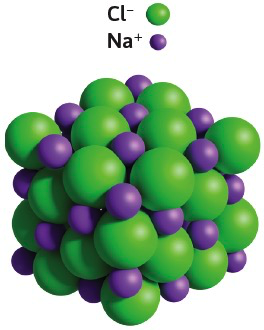
\includegraphics[width=0.5\textwidth]{ionicos1.jpg}
        \captionof{figure}{ Representación nanoscópica del cloruro de sodio (NaCl).}
        \label{fig:ionicos1}
    \end{figure}
\end{minipage}\hfill
\begin{minipage}{0.45\textwidth}
    \begin{figure}[H]
        \centering
        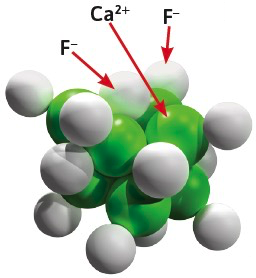
\includegraphics[width=0.5\textwidth]{ionicos2.jpg}
        \captionof{figure}{ Representación nanoscópica del fluoruro de calcio (CaF$_2$).}
        \label{fig:ionicos2}
    \end{figure}
\end{minipage}

Los compuestos iónicos, como la sal común (cloruro de sodio, NaCl), resultan de la combinación de
átomos de elementos no metálicos y átomos de elementos metálicos. En general, los átomos de los
elementos metálicos son más grandes que los de elementos no metálicos. Esto causa que los
electrones de valencia de los átomos metálicos estén más alejados del núcleo y se muevan con
más facilidad que los de los no metales. De hecho, cuando átomos de elementos metálicos
interaccionan con los de no metales, los electrones de valencia de los metales se transfieren a
los no metales. En este proceso, los átomos de los metales se transforman en cationes mientras
los de los no metales forman aniones.

Considera, por ejemplo, la interacción entre átomos de sodio (Na, Z = 11, metálico) y de cloro
(Cl, Z = 17, no metálico). En este proceso los átomos de sodio pierden un electrón de valencia
y forman cationes Na$^+$, mientras que los de cloro ganan un electrón de valencia adicional y forman
aniones Cl$^-$. Cuando un trozo de sodio metálico se pone en contacto con una muestra de cloro se
producen millones de iones Na$^+$ y Cl$^-$. Dado que cargas de signos opuestos se atraen, los iones
Na$^+$ y Cl$^-$ forman un conglomerado de iones (red iónica) en el que cada ion está rodeado por iones de signo opuesto (figura 2.25). Esta red es muy estable y el compuesto químico que se forma es el famoso cloruro de sodio, cuya fórmula se representa como NaCl. Es importante destacar que esta fórmula no indica que esta sustancia está constituida por moléculas con un ion de sodio y uno de cloro , sino que en la red tiene miles de iones, y por cada ion de Na+ hay un ion de Cl$^-$.

El mismo modelo se puede utilizar para explicar y predecir la formación de otros compuestos iónicos.
Considera la interacción entre átomos de calcio (Ca, Z = 20, metálico) y de flúor (F, Z = 9, no
metálico). Los átomos de calcio tienden a perder sus dos electrones de valencia cuando interaccionan
con átomos de elementos no metálico como el flúor y, por tanto, se forman cationes Ca2$^+$.
Sin embargo, cada átomo no metálico de flúor sólo es capaz de aceptar un electrón para formar
aniones F$^-$. Como cada átomo de calcio transfiere dos electrones, uno solo de estos átomos
transforma dos de flúor en dos iones fluoruro, F$^-$. Cuando los millones de iones que se generan
interaccionan entre sí, se forma una red iónica en la que hay dos aniones F$^-$ por cada
catión Ca2$^+$. El compuesto iónico que se produce se llama fluoruro de calcio, y su fórmula
condensada es, entonces, CaF$_2$ (en la fórmula el elemento metálico siempre se representa primero)
(figura \ref{fig:ionicos2}).\\

\begin{boxK}
    Infiere, representa e investiga
    \begin{enumerate}
        \item Identifica la fórmula condensada del compuesto iónico que se forma al combinar cada par
              de elementos listados en esta tabla.
              \begin{figure}[H]
                  \centering
                  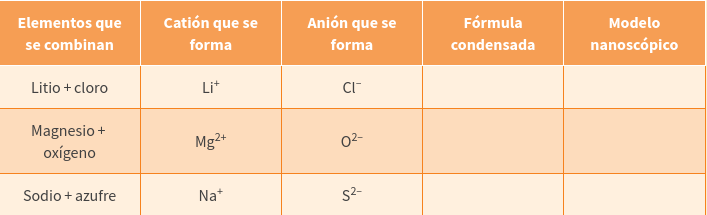
\includegraphics[width=0.8\textwidth]{tabla_ionicos.png}
                  \label{fig:tabla_ionicos}
              \end{figure}
        \item Construyan en equipos un modelo de cada compuesto iónico a nivel nanoscópico. Representen la proporción de cada ion en la red iónica.
        \item Investiguen los usos comunes de los compuestos iónicos que se forman.
    \end{enumerate}
\end{boxK}

En general, la fuerza de atracción que mantiene unidos a los iones en compuestos iónicos es grande,
lo cual hace que no se separen con facilidad. Es por ello que estos compuestos tienden a ser sólidos
con altos puntos de fusión, pues es necesario proporcionar gran cantidad de energía para que los
iones se separen y adquieran movilidad.

\begin{boxK}
    \begin{enumerate}
        \item  Analiza el modelo y úsalo para explicar que los compuestos iónicos son sólidos y que se fragmentan con facilidad al golpearlos.
              \begin{figure}[H]
                  \centering
                  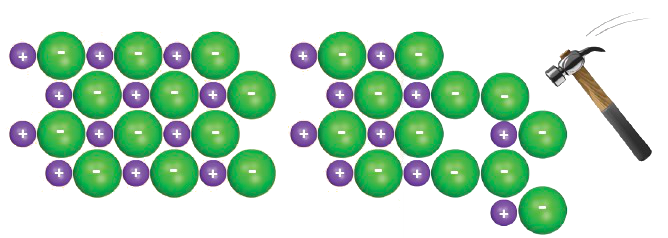
\includegraphics[width=0.6\textwidth]{ionicos3.png}
                  \label{fig:ionicos3}
              \end{figure}
        \item Comenta tus ideas con tus compañeros y corríjanlas en caso de ser necesario.
    \end{enumerate}
\end{boxK}

\begin{boxK}
    \begin{enumerate}
        \item Analiza cada representación de distintas sustancias y determina qué tipo de sustancia (molecular, metálica o iónica) se busca representar.
              \begin{figure}[H]
                  \centering
                  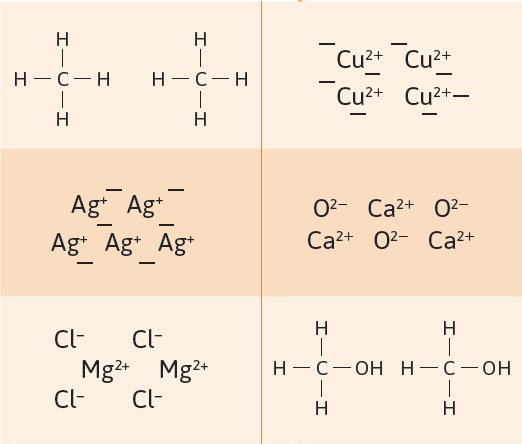
\includegraphics[width=0.6\textwidth]{formulas_condensadas.jpg}
              \end{figure}
        \item Escribe la fórmula condensada de cada una.
        \item Predice las propiedades físicas de esas sustancias, luego investígalas en libros e internet y contrástalas con tus predicciones.
        \item Haz una representación similar a las anteriores de tres sustancias de la actividad del inicio de esta lección y menciona a qué tipo de sustancia corresponde cada grupo que se incluyó en la tabla.
        \item Comparte tus predicciones con tus compañeros de clase y justifícalas con base en la composición y estructura de las distintas sustancias.
    \end{enumerate}
\end{boxK}

\subsubsection{Ejercicios}

\begin{boxK}
    Relaciona el catión y anión que forman el compuesto:\\

    \begin{minipage}{0.5\textwidth}
        \begin{enumerate}
            \item Cloruro de potasio (KCl)
            \item Óxido de magnesio (MgO)
            \item Sulfuro  de sodio (Na2S)
            \item Yoduro de potasio (Kl)
            \item Bromuro de potasio (KBr)
            \item Óxido de hierro (FeO)
            \item Cloruro de potasio  (KCl)
            \item Óxido de calcio (CaO)
            \item Fluoruro de litio (LiF)
            \item Cloruro de berilio (BeCl$_2$)
            \item Fluoruro de sodio (NaF)
            \item Óxido de bario (BaO)
            \item Yoduro de rubidio (Rbl)
            \item Sulfuro de aluminio (Al$_2$S$_3$)
            \item Bromuro de sodio (NaBr)
        \end{enumerate}
    \end{minipage}%
    % \vspace{2cm}
    \begin{minipage}{0.5\textwidth}
        \begin{itemize}
            \item[\rule{1cm}{0.2mm}] Ca$^{2+}$O$^{2-}$
            \item[\rule{1cm}{0.2mm}] K$^+$Br$^-$
            \item[\rule{1cm}{0.2mm}] Mg$^{2+}$O$^{2-}$
            \item[\rule{1cm}{0.2mm}] Fe$^{2+}$O$^{2-}$
            \item[\rule{1cm}{0.2mm}] K$^+$I$^-$
            \item[\rule{1cm}{0.2mm}] K$^+$Cl$^-$
            \item[\rule{1cm}{0.2mm}] K$^+$Cl$^-$
            \item[\rule{1cm}{0.2mm}] Na$^+$S$^{2-}$
            \item[\rule{1cm}{0.2mm}] Ba$^{2+}$+O$^{2-}$
            \item[\rule{1cm}{0.2mm}] Al$^{3+}$S$^{2-}$
            \item[\rule{1cm}{0.2mm}] Be$^{2+}$+Cl$^{-}$
            \item[\rule{1cm}{0.2mm}] Na$^+$Br$^-$
            \item[\rule{1cm}{0.2mm}] Rb$^+$I$^-$
            \item[\rule{1cm}{0.2mm}] Li$^+$F$^-$
            \item[\rule{1cm}{0.2mm}] Na$^+$F$^-$
        \end{itemize}
    \end{minipage}
\end{boxK}

\begin{boxK}
    Relaciona cada elemento con las características que le corresponden.

    \begin{minipage}{0.6\textwidth}
        \begin{enumerate}\footnotesize
            \item Elemento del grupo VII, con siete electrones en la última capa de valencia, ubicado en el tercer periodo de la tabla periódica.
            \item Elemento metaloide, ubicado en el tercer periodo de la tabla periódica.
            \item Elemento conocido como gas noble.
            \item Elemento metálico con Z = 11.
            \item Elemento que se ubica en el grupo 15 y en el periodo 2 de la tabla periódica.
            \item Elemento con 12 protones y 12 electrones.
            \item Elemento no metálico con Z =34
            \item Ejemplo de gas inerte.
        \end{enumerate}
    \end{minipage}\hfill
    \begin{minipage}{0.25\textwidth}
        \begin{itemize}
            \item[\rule{1cm}{0.2mm}] Selenio
            \item[\rule{1cm}{0.2mm}] Neón
            \item[\rule{1cm}{0.2mm}] Magnesio
            \item[\rule{1cm}{0.2mm}] Xenón
            \item[\rule{1cm}{0.2mm}] Sodio
            \item[\rule{1cm}{0.2mm}] Cloro
            \item[\rule{1cm}{0.2mm}] Nitrógeno
            \item[\rule{1cm}{0.2mm}] Silicio
        \end{itemize}
    \end{minipage}
\end{boxK}
\begin{boxK}
    Relaciona cada elemento con las características que le corresponden.

    \begin{minipage}{0.6\textwidth}
        \begin{enumerate}\footnotesize
            \item Elemento con cuatro electrones en su última capa de valencia.
            \item Ejemplo de gas noble.
            \item Elemento de la familia de metales alcalinos.
            \item Metal brillante utilizado en joyería.
            \item Líquido rojo oscuro.
            \item Gas incoloro que arde en presencia de oxígeno.
            \item Metal reactivo que reacciona fácilmente con agua.
        \end{enumerate}
    \end{minipage}\hfill
    \begin{minipage}{0.25\textwidth}
        \begin{itemize}
            \item[\rule{1cm}{0.2mm}] Neón
            \item[\rule{1cm}{0.2mm}] Bromo
            \item[\rule{1cm}{0.2mm}] Calcio
            \item[\rule{1cm}{0.2mm}] Oro
            \item[\rule{1cm}{0.2mm}] Rubidio
            \item[\rule{1cm}{0.2mm}] Hidrógeno
            \item[\rule{1cm}{0.2mm}] Carbono
        \end{itemize}
    \end{minipage}
\end{boxK}

% \begin{boxK}  Relaciona los siguientes elementos:\\
%   \begin{minipage}{0.5\textwidth}
%     \begin{enumerate}

%     \end{enumerate}
%   \end{minipage}%
%   \begin{minipage}{0.5\textwidth}
%     \begin{itemize}

%     \end{itemize}
%   \end{minipage}
% \end{boxK}

\newpage \thispagestyle{plain}
\section{Moléculas de importancia para la vida}
\boxabstract{Aprendizajes esperados:}{
    \begin{itemize}
        \item Identifica componentes químicos importantes
              (carbohidratos, lípidos, proteínas, ADN) que participan en
              la estructura y funciones del cuerpo humano.
        \item Representa y diferencia mediante esquemas, modelos y
              simbología química, elementos y compuestos, así como
              átomos y moléculas.
        \item Explica y predice propiedades físicas de los materiales
              con base en modelos submicroscópicos sobre la
              estructura de átomos, moléculas o iones, y sus
              interacciones electrostáticas.
    \end{itemize}
}

\subsection{¿Qué moléculas nos constituyen?}

\newpage